\documentclass[10pt, UKenglish]{exam}
\usepackage[UKenglish]{babel} 
\usepackage[]{fontspec} 
\usepackage[]{amsmath,amssymb}
\usepackage[]{mathtools} 
\usepackage[]{cleveref} 
\usepackage[]{greekctr} 
\usepackage[]{cancel} 
\usepackage[]{lipsum} 
\usepackage[]{csquotes} 
\usepackage[]{isodate} 
\usepackage[]{siunitx}
\usepackage[]{textcomp} 
\usepackage[]{tabularx} 
\usepackage[]{pdflscape} 
\usepackage[]{xcolor} 
\usepackage[]{enumitem} 
\usepackage[]{calc} 
\usepackage[normalem]{ulem} 
\usepackage[]{arydshln} 
\usepackage[]{subcaption} 
\graphicspath{{figures}}

% siunitx - numeric formatting
\DeclareSIUnit[]{\SIeuro}{€}
\newcommand{\price}[1]{\SI[round-precision=2,round-mode=places]{#1}[]{\SIeuro}}
\newcommand{\weight}[1]{\qty{#1}{\gram}}
\newcommand{\dimensions}[1]{\qtyproduct{#1}{\milli\metre}}
\newcommand{\displaysize}[1]{\qty{#1}{"}}
\newcommand{\capacity}[1]{\qty{#1}{\milli\ampere\hour}}

% cleverref - exam cls
\renewcommand\partlabel{(\alph{partno})}
\renewcommand\subpartlabel{(\roman{subpart})}
\renewcommand\subsubpartlabel{(\greek{subsubpart})}

\crefname{question}{question}{questions}
\crefname{subpart}{part}{parts}
\crefname{subsubpart}{part}{parts}
\crefname{partno}{part}{part}
\creflabelformat{question}{(#2#1#3)}
\creflabelformat{subpart}{(#2#1#3)}
\creflabelformat{subsubpart}{(#2#1#3)}
\creflabelformat{partno}{(#2#1#3)}

\begin{document}

\title{AOS4 - Smartphone purchase}
\author{Pascal Quach}
\maketitle

Your parents have decided to buy you a new smartphone, and ask you to choose
among  a list they have prepared for you. Unfortunately for you, you tend to be
\textbf{very thorough} when choosing your smartphone, but cannot actually change the list
without your parents' approval.

Stuck with a fixed list, you resolve yourself to make the best decision
according to your tastes. Fortunately, you have been studying multi-criteria
decision-making (MCDM), what a coincidence!

After consulting with your parents, they give you the following guidelines:

\begin{enumerate}
	\item \textquote{The price cannot exceed \price{1000}}
	\item \textquote{The camera or chipset should not influence your
		decision}
	\item \textquote{It is preferable if you give a ranking, rather than a
		choice}
\end{enumerate}

After searching for the products' details online, you compile the information into~\cref{tab:em-1}

\begin{comments}
	This exercise should be solved in class, as practice for MCDM.
	The familiar context enables students to confront their own
	reasoning to the studied decision theory, and facilitates
	reviewing taken decisions.
	The questions let students identify the types of criteria
	(order/type), apply Pareto Dominance, lexicographic/WS
	aggregation, normalization for aggregation, and further
	identify the different elicitation scenarios.
	The evaluation matrix does not include technical details to
	reduce the amount of assumed technical knowledge.
\end{comments}

\begin{questions}
	\question
	
	\begin{parts}
		\part \label{q:1a}%
		According to your preferences, and only using the criteria 
		contained in~\cref{tab:em-1}, make a decision and list your top
		3 choices.
		\part \label{q:1b}% 
		For each criterion, answer the following questions, and compare your
		answers in group:
		
		\begin{subparts}
			\subpart \label{q:1bi}%
			What objective have you chosen, \textit{e}.\textit{g}.\
			$\max$, $\min$?

			\subpart \label{q:1bii}%
			If you cannot choose an objective, how did you order
			the values?
			
			\subpart \label{q:1biii}%
			Are there criteria that are \textquote{not important},
			\textit{i}.\textit{e}.\ for which you have no
			preference?
		\end{subparts}
	\end{parts}

	\begin{comments}
		Introductory question, familiarize with the context
		and the data. Identify subjective aspects of the criteria,
		types of criteria, etc.

		For~\cref{q:1a}, the idea is to introduce the data to the 
		student, and make sure he has gone through the table. Any preferences
		the student has can serve for further reasoning. Why did they prefer
		certain criteria to others? Which objectives did they choose for each
		criterion?

		In~\cref{q:1b}, criteria are studied more in depth and is directly
		following the previous line of thought, but explicitly.
	\end{comments}
	
	\begin{solutionorbox}

		A suggested solution is the following:

		\begin{enumerate}
			\item[(a)] Google Pixel 7 Pro, Samsung Galaxy A52s 5G, Nothing Phone (1)
			\item [(b)] \begin{enumerate}
				\item (Brand) Google, Samsung, OnePlus, Nothing, \sout{Apple/Xiaomi/Asus/Huawei/Motorola}
				\item (Release Date) No preference
				\item (Dimensions) No preference
				\item (5G) No preference
				\item (Display Type) All the values indicated are identical
				\item (Display Size) Maximum
				\item (Operating System) Android, \sout{iOS/EMUI}
				\item (Jack) No preference
				\item (Battery capacity) Maximize
				\item (Price) Minimize
			\end{enumerate}
		\end{enumerate}
		
	\end{solutionorbox}
	
	\question\label{q:2}%
	Using the criteria that you identified as relevant, try to apply Pareto
	Dominance to make a decision.

	\begin{comments}
		Practice question for Pareto Dominance. Results might vary from
		individual to individual. The TA may instead choose a fixed
		list of  interesting criteria, e.g. 5G, jack, display size,
		operating system, battery capacity, and price.

		Almost certainly, students will showcase conflicting
		objectives, \textit{e}.\textit{g}.\ minimize price and maximize
		battery capacity.
	\end{comments}
	
	\begin{solutionorbox}
		Using brand, display size, operating system, battery capacity and price:

		{
			\footnotesize
			\begin{tabular}{|c|c|c|c|c|c|}
							\hline
				Name & Brand & Display Size & Operating System & Battery capacity & Price \\%&
				\hdashline
				Objective & Ordered & Maximize & Ordered & Maximize & Minimize \\
				\hline\hline
				Google Pixel 7 Pro & Google & \displaysize{6.7} & Android & \capacity{5000} & \price{812.00}\\%&
				\hline
				Samsung Galaxy A52s 5G & Samsung & \displaysize{6.5} & Android & \capacity{4500} & \price{349.99}\\%&
				\hline
				Samsung Galaxy S22 Ultra 5G & Samsung & \displaysize{6.8} & Android & \capacity{5000} & \price{928.00}\\%&
				\hline
				OnePlus 10 Pro & OnePlus & \displaysize{6.7} & Android & \capacity{5000} & \price{724.99}\\%&
				\hline
				Nothing Phone (1) & Nothing & \displaysize{6.55} & Android & \capacity{4500} & \price{399.00}\\%&
				\hline
				Asus Zenfone 9 & \sout{Asus} & \displaysize{5.9} & Android & \capacity{4300} & \price{743.89}\\%&
				\hline
				Asus ROG Phone 6D Ultimate & \sout{Asus} & \displaysize{6.78} & Android & \capacity{6000} & \price{1399.00}\\%&
				\hline
				Huawei Mate 50 Pro & \sout{Huawei} & \displaysize{6.74} & \sout{EMUI} & \capacity{4700} & \price{1154.99}\\%&
				\hline
				Xiaomi 11T Pro & \sout{Xiaomi} & \displaysize{6.67} & Android & \capacity{5000} & \price{412.99}\\%&
				\hline
				Xiaomi 12 Pro & \sout{Xiaomi} & \displaysize{6.73} & Android & \capacity{4600} & \price{758.00}\\%&
				\hline
				Motorola Moto X40 & \sout{Motorola} & \displaysize{6.7} & Android & \capacity{4600} & \price{465.79}\\%&
				\hline
				Apple iPhone 13 Pro Max & \sout{Apple} & \displaysize{6.7} & \sout{iOS} & \capacity{4352} & \price{1379}\\%&
				\hline
			\end{tabular}
		}

		We sorted the table by brand, meaning that a phone cannot be
		Pareto-dominated by a lower one of a different brand. Brands
		that are not considered are eliminated from the alternatives.

		As such, we begin from eligible products from the top to
		eliminate dominated alternatives:

		\begin{itemize}
			\item The Google Pixel 7 Pro is at least beaten by
				lower alternatives on price, display size,
				price, and price respectively.
			\item The Samsung Galaxy A52s 5G is beaten by lower alternatives on display size.
			\item The Samsung Galaxy S22 Ultra 5G is beaten by lower alternatives on price.
			\item The OnePlus 10 Pro is beaten by lower alternatives on price.
		\end{itemize}

		There are no Pareto dominance relationships.
	\end{solutionorbox}

	\question\label{q:3}%
	You have been probably unable to apply Pareto dominance relationships
	to eliminate alternatives. 

	\begin{parts}\label{q:3a}%
		\part\label{q:3ai}%
		Try to think of reasons why, and write them down. \textit{Hint:
		are your criteria completely independent from each other?} 

		\part\label{q:3aii}%
		Which method would be suitable to solve this decision problem,
		if you were making a choice?
	\end{parts}

	\begin{solutionorbox}
		Some objectives might be conflicting, meaning that you cannot
		at the same time maximize display size, battery capacity and
		minimize the price.

		One alternative method to solve this problem could be even
		swaps, as you resolve the trade-offs by trading criteria for
		others, \textit{e}.\textit{g}.\ \qty{500}{\milli\ampere\hour}
		might be traded for \price{100}.
	\end{solutionorbox}

	\question\label{q:4}%
	As you are unable to rank the products using Pareto optimization
	techniques, you decide to merge the criteria together. For that, you
	believe both lexicographic and weighted sum aggregation are appropriate
	techniques, and you wish to compare the results.

	\begin{parts}
		\part\label{q:4a}%
		Use lexicographic aggregation. What issues does this method have?

		\part\label{q:4b}%
		Use weighted sum aggregation. What issues does this method have?
	\end{parts}
	
	\begin{comments}
		The question introduces aggregation techniques for practice
		purposes. Optionally, the Choquet Integral can be introduced. 

		For the lexicographic aggregation, the students must first rank
		the criteria, then solve the problem. As for issues, serial
		\textbf{dictactorship} prioritizes certain criteria over
		others. Given the limited list, if the student prefers a Google
		phone over all other brands, then they only have a single
		choice, regardless of all other criteria.

		For the weighted sum aggregation, the students must assign
		numeric values to each criterion, then also convert the
		symbolic criteria to numeric ones, \textit{e}.\textit{g}.\ by
		ranking, and finally solve the problem. The critical issues
		here are to appropriately convert symbolic criteria to numeric
		ones, and objectives to the same one (either minimize or
		maximize). A further issue is the difference in numeric range
		for different criteria. Preferably, the student should
		\textbf{normalize} values first.
	\end{comments}
	
	\begin{solutionorbox}
		An example would be the following:

		For~\cref{q:4a}, brand is prioritized first, thus the only choice is the Google Pixel 7 Pro.
			
		For ~\cref{q:4b}, the weights for brand, display size, battery capacity and price are respectively: 
				\qty{0.2}, \qty{0.2}, \qty{0.3}, \qty{0.3}.
			
		Unnormalized scores are:
		\[
			\small
			\begin{aligned}
				\text{Score(Google Pixel 7 Pro)} &\coloneqq 0.2\times 4 + 0.2\times 6.7 + 0.3\times 5000 - 0.3\times 812.00 = 1258.54\\
				\text{Score(Samsung Galaxy A52s 5G)} &\coloneqq 0.2\times 3 + 0.2\times 6.5 + 0.3\times 4500 - 0.3\times 349.99 = 1246.90\\
				\text{Score(Samsung Galaxy S22 Ultra 5G)} &\coloneqq 0.2\times 3 + 0.2\times 6.8 + 0.3\times 5000 - 0.3\times 928.00 = 1223.56\\
				\text{Score(OnePlus 20 Pro)} &\coloneqq 0.2\times 3 + 0.2\times 6.7 + 0.3\times 5000 - 0.3\times 724.99 = 1284.44\\
				\text{Score(Nothing Phone (1))} &\coloneqq 0.2\times 1 + 0.2\times 6.55 + 0.3\times 4500 - 0.3\times 399.00 = 1231.155\\
			\end{aligned}
		.\] 

		The ranking is thus: OnePlus 20 Pro, Google Pixel 7 Pro, Samsung Galaxy A52s 5G, Nothing Phone (1), Samsung Galaxy S22 Ultra 5G.

		If we normalize (mean/variance) the scores using all data from~\cref{tab:em-1}, then:
		\[
			\small
			\begin{aligned}
				\text{Score*(Google Pixel 7 Pro)} &\coloneqq 0.5951\\
				\text{Score*(Samsung Galaxy A52s 5G)} &\coloneqq 0.3392\\
				\text{Score*(Samsung Galaxy S22 Ultra 5G)} &\coloneqq 0.4428\\
				\text{Score*(OnePlus 20 Pro)} &\coloneqq 0.3920\\
				\text{Score*(Nothing Phone (1))} &\coloneqq 0.0625\\ 
			\end{aligned}
		.\] 

		The final ranking is Google Pixel 7 Pro, Samsung Galaxy S22
		Ultra 5G, OnePlus 20 Pro, Samsung Galaxy A52s 5G, and Nothing
		Phone (1).

		The results are remarkably different between unnormalized and
		normalized data. Although, the Google Pixel 7 Pro is still
		chosen by both lexicographic and weighted sum models. 
	\end{solutionorbox}
	
	\question\label{q:5}%
	Do you agree with the decision made using aggregation? Why? 
	
	\begin{parts}
		\part\label{q:5a}
		Are the ranking coherent with your preferences?

		\part\label{q:5b}%
		How did you rank the criteria? How did you estimate the
		weights?

		\part\label{q:5c}%
		Suggest a better aggregation procedure.

	\end{parts}
	
	\begin{comments}
		The question aims at providing more insight into how exactly
		the aggregation chose to rank the alternatives, and which
		criteria took the most importance. The students must realize
		that there exists a lot of subjectivity into how the criteria
		are aggregated, and also difficulties in the aggregation
		itself. 
	\end{comments}
	
	\begin{solutionorbox}
		The lexicographic is too drastic, the WS aggregation is linear,
		the student must suggest a better aggregation method.

		It is not asked that students define a fuzzy measure for this
		problem, but they should mention the Choquet, or the Sugeno
		integral.
	\end{solutionorbox}
	
	\question\label{q:6}%
	After a very long and arduous decision process, you finally have a
	ranking of potential smartphones, albeit with some faults! 

	However, you cannot afford to spend more time on this, and decide to
	examine the final criterion: the design!

	You group together all the visuals in~\cref{fig:smartphones-design}.

	\begin{parts}
		\part\label{q:6a}%
		Which products matches your tastes the best? Rank them.
		
		\part\label{q:6b}%
		Compare your tastes with your class, by counting who likes
		which products. Can you identify clusters of similar products?

		\part\label{q:6c}%
		If you had to assign a cause to these clusters, what would they
		be? Discuss.

	\end{parts}

	\begin{comments}
		Introduce a very subjective visual criteria, which can be
		thought as a MCDM problem in itself.
	\end{comments}
	
	\begin{solutionorbox}
		One example answer: 
		\begin{itemize}
			\item g, h, k, l, j, f, a, d, c, b, i, e
			\item In practice, just fill in a matrix
				students/products. Hopefully, there should be
				some groups of products easily identifiable.
			\item This is a discussion on the cause of natural
				clustering in
				smartphones. Some causes might be: design
				features, \textit{e}.\textit{g}.\ notches, back
				cameras, etc., product personality, brand, etc.
		\end{itemize}

		The discussion should naturally evolve into listing a number of
		criteria for choosing the design, resulting in making the final
		criterion a MCDM problem in itself. 

		Collecting users' preferences is a very difficult task.
	\end{solutionorbox}
\end{questions}

\begin{figure*}[htpb]
	\captionsetup[subfigure]{justification=centering}
	\centering
	\begin{subfigure}[htpb]{0.25\linewidth}
	\begin{center}
		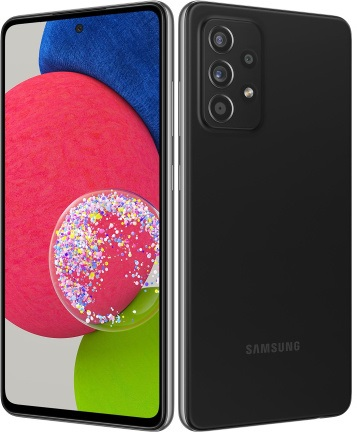
\includegraphics[width=\linewidth,height=4cm,keepaspectratio]{samsung-galaxy-a52s-5g}
	\end{center}
	\caption{Samsung Galaxy A52s 5G}
	\label{fig:samsung-galaxy-a52s-5g}
	\end{subfigure}
	\begin{subfigure}[htpb]{0.25\linewidth}
	\begin{center}
		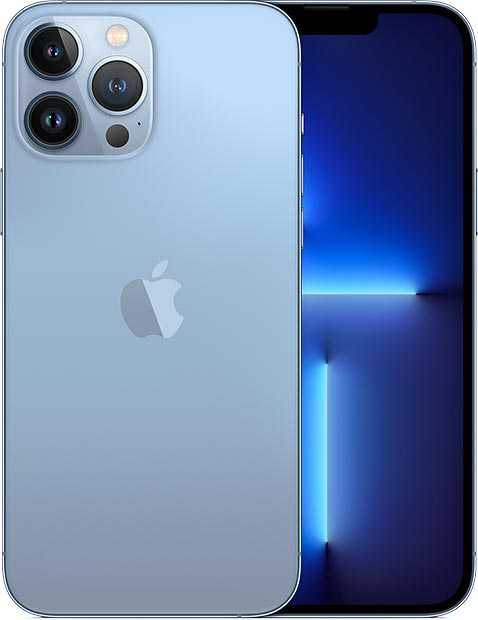
\includegraphics[width=\linewidth,height=4cm,keepaspectratio]{apple-iphone-13-pro-max}
	\end{center}
	\caption{Apple iPhone 13 Pro Max}
	\label{fig:apple-iphone-13-pro-max}
	\end{subfigure}
	\begin{subfigure}[htpb]{0.25\linewidth}
	\begin{center}
		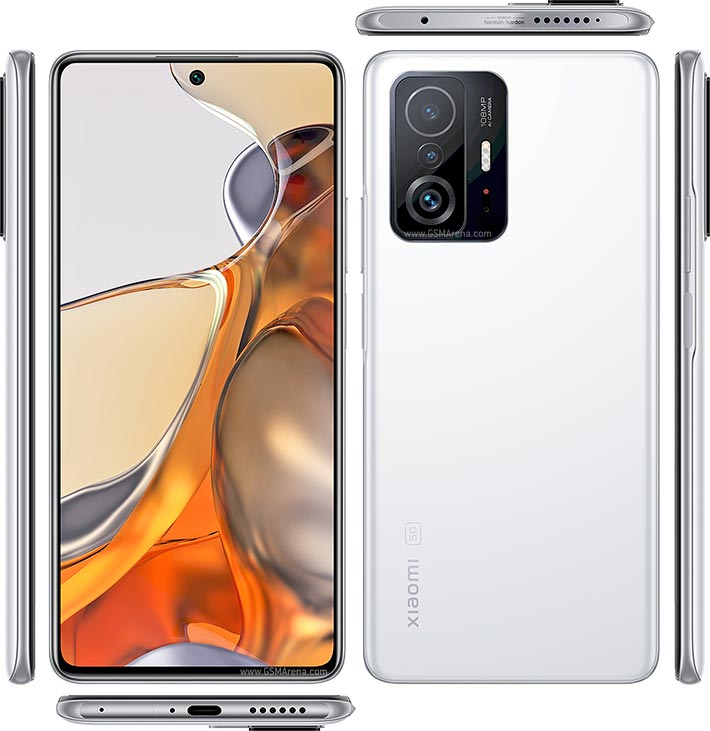
\includegraphics[width=\linewidth,height=4cm,keepaspectratio]{xiaomi-11t-pro}
	\end{center}
	\caption{Xiaomi 11T Pro}
	\label{fig:xiaomi-11t-pro}
	\end{subfigure}

	\begin{subfigure}[htpb]{0.25\linewidth}
	\begin{center}
		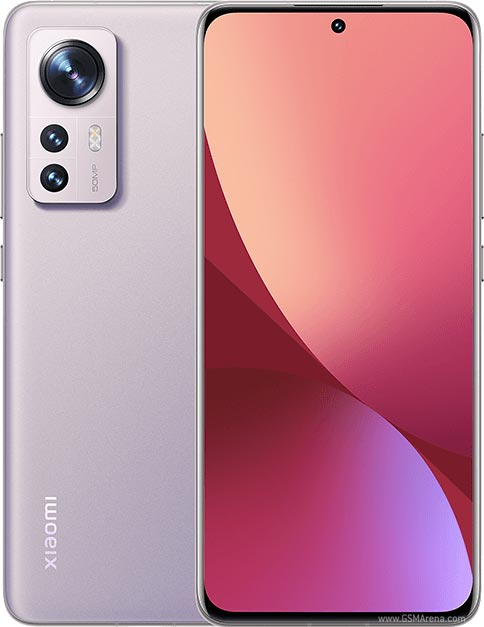
\includegraphics[width=\linewidth,height=4cm,keepaspectratio]{xiaomi-12-pro}
	\end{center}
	\caption{Xiaomi 12 Pro}
	\label{fig:xiaomi-12-pro}
	\end{subfigure}
	\begin{subfigure}[htpb]{0.25\linewidth}
	\begin{center}
		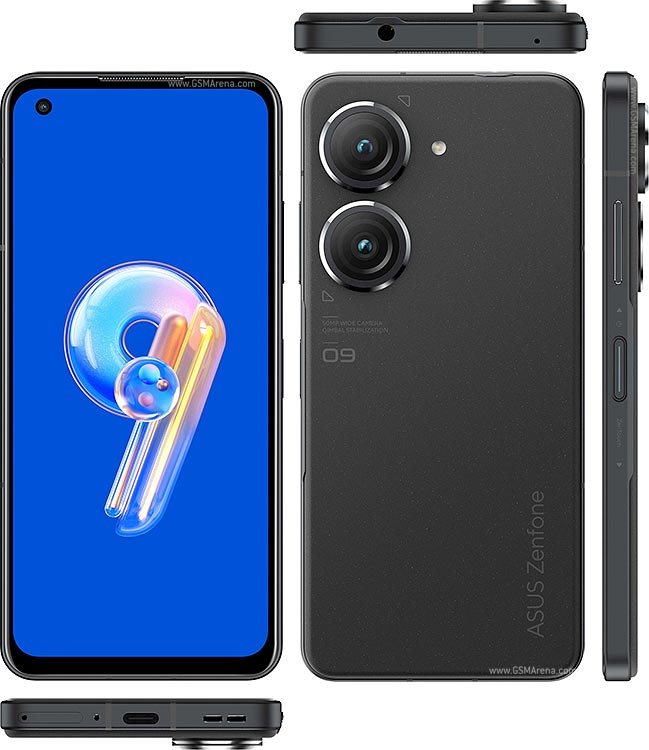
\includegraphics[width=\linewidth,height=4cm,keepaspectratio]{asus-zenfone-9}
	\end{center}
	\caption{Asus Zenfone 9}
	\label{fig:asus-zenfone-9}
	\end{subfigure}
	\begin{subfigure}[htpb]{0.25\linewidth}
	\begin{center}
		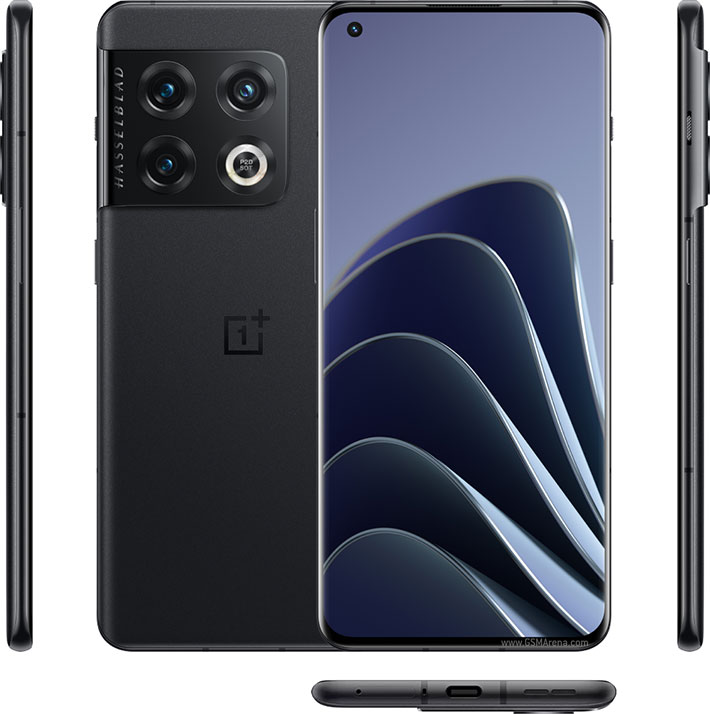
\includegraphics[width=\linewidth,height=4cm,keepaspectratio]{oneplus-10-pro}
	\end{center}
	\caption{OnePlus 10 Pro}
	\label{fig:oneplus-10-pro}
	\end{subfigure}

	\begin{subfigure}[htpb]{0.25\linewidth}
	\begin{center}
		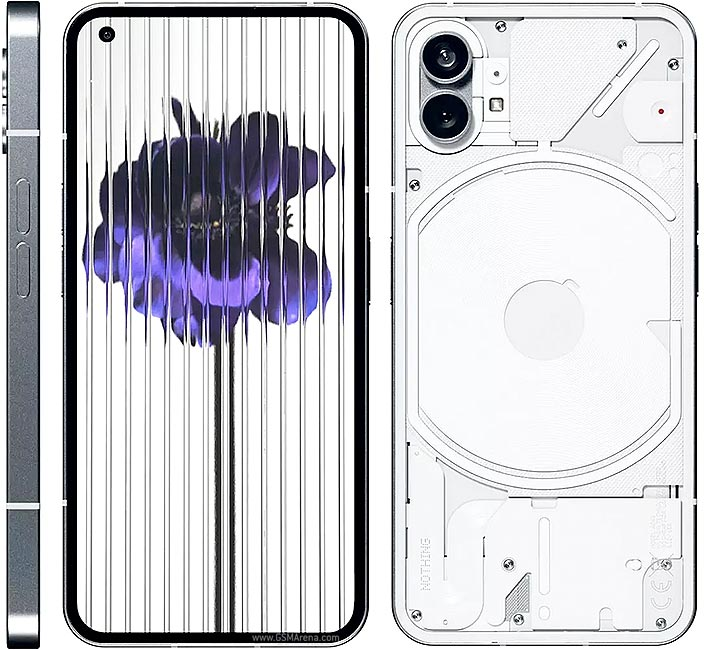
\includegraphics[width=\linewidth,height=4cm,keepaspectratio]{nothing-phone-1}
	\end{center}
	\caption{Nothing Phone (1)}
	\label{fig:nothing-phone-1}
	\end{subfigure}
	\begin{subfigure}[htpb]{0.25\linewidth}
	\begin{center}
		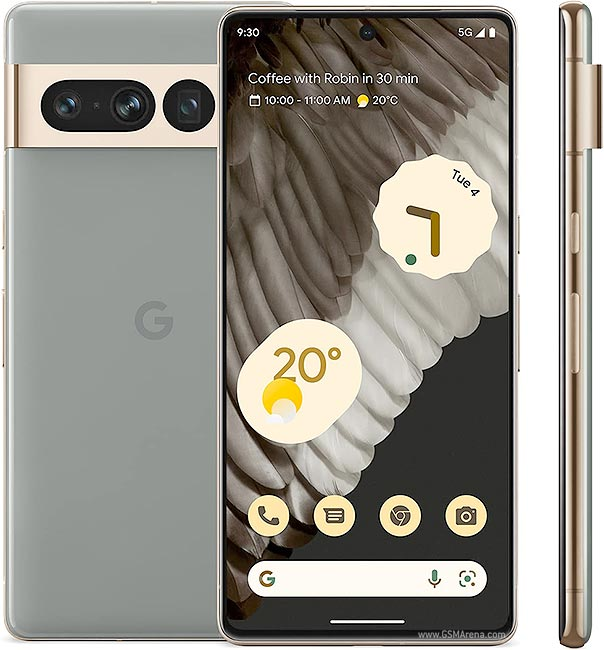
\includegraphics[width=\linewidth,height=4cm,keepaspectratio]{google-pixel-7-pro}
	\end{center}
	\caption{Google Pixel 7 Pro}
	\label{fig:google-pixel-7-pro}
	\end{subfigure}
	\begin{subfigure}[htpb]{0.25\linewidth}
	\begin{center}
		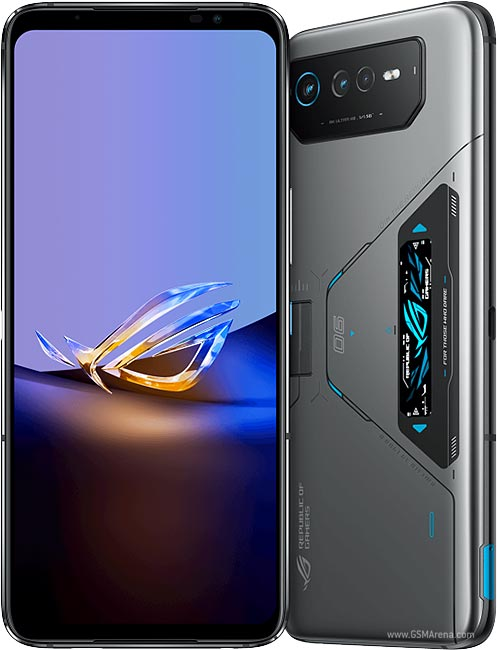
\includegraphics[width=\linewidth,height=4cm,keepaspectratio]{asus-rog-phone-6d-ultimate}
	\end{center}
	\caption{Asus ROG Phone 6D Ultimate}
	\label{fig:asus-rog-phone-6d-ultimate}
	\end{subfigure}

	\begin{subfigure}[htpb]{0.25\linewidth}
	\begin{center}
		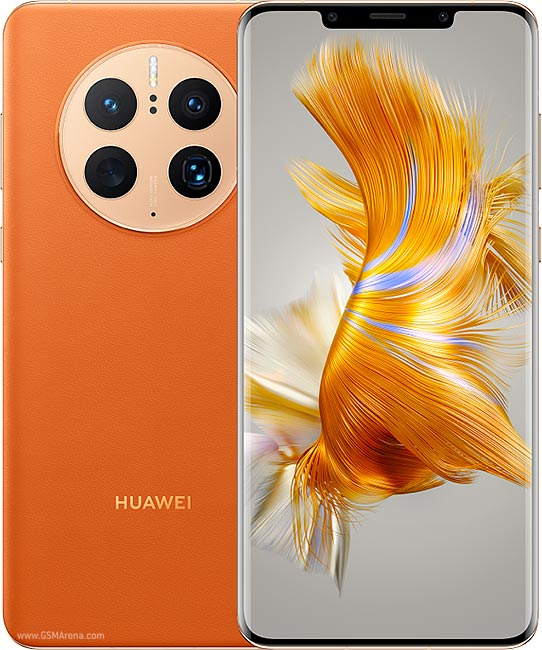
\includegraphics[width=\linewidth,height=4cm,keepaspectratio]{huawei-mate-50-pro}
	\end{center}
	\caption{Huawei Mate 50 Pro}
	\label{fig:huawei-mate-50-pro}
	\end{subfigure}
	\begin{subfigure}[htpb]{0.25\linewidth}
	\begin{center}
		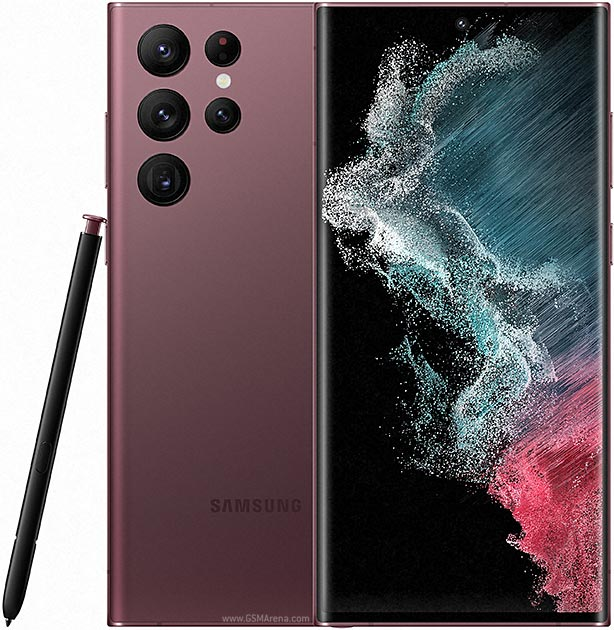
\includegraphics[width=\linewidth,height=4cm,keepaspectratio]{samsung-galaxy-s22-ultra-5g}
	\end{center}
	\caption{Samsung Galaxy S22 Ultra 5G}
	\label{fig:samsung-galaxy-s22-ultra-5g}
	\end{subfigure}
	\begin{subfigure}[htpb]{0.25\linewidth}
	\begin{center}
		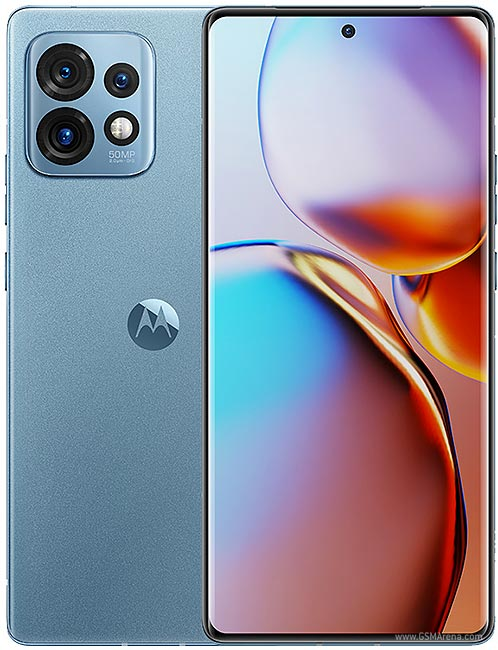
\includegraphics[width=\linewidth,height=4cm,keepaspectratio]{motorola-moto-x40}
	\end{center}
	\caption{Motorola Moto X40}
	\label{fig:motorola-moto-x40}
	\end{subfigure}
	
	\caption{Smartphones Designs}
	\label{fig:smartphones-design}
\end{figure*}


\begin{landscape}
\begin{table*}[htpb]
	\centering
	\caption{Smartphones details}
	
	\scriptsize
	\label{tab:em-1}	
	\begin{tabularx}{24.5cm}{|X|X|X|X|X|X|X|X|X|X|X|X|}
		\hline
		Name & Brand & Release Date & Dimensions & Weight & 5G & Display Type & Display Size & Operating System & \qty{3.5}{\milli\meter} Jack & Battery capacity & Price \\%&
		\hline\hline
		Samsung Galaxy A52s 5G & Samsung & \printdate{01/09/2021} & \dimensions{159.9 x 75.1 x 8.4} & \weight{189} & Yes & OLED & \displaysize{6.5} & Android & Yes & \capacity{4500} & \price{349.99}\\%&
		\hline
		Apple iPhone 13 Pro Max & Apple & \printdate{24/09/2021} & \dimensions{160.8 x 78.1 x 7.7} & \weight{240} & Yes & OLED & \displaysize{6.7} & iOS & No & \capacity{4352} & \price{1379}\\%&
		\hline
		Xiaomi 11T Pro & Xiaomi & \printdate{05/10/2021} & \dimensions{164.1 x 76.9 x 8.8} & \weight{204} & Yes & OLED & \displaysize{6.67} & Android & No & \capacity{5000} & \price{412.99}\\%&
		\hline
		Xiaomi 12 Pro & Xiaomi & \printdate{31/12/2021} & \dimensions{163.6 x 74.6 x 8.2} & \weight{204} & Yes & OLED & \displaysize{6.73} & Android & No & \capacity{4600} & \price{758.00}\\%&
		\hline
		Asus Zenfone 9 & Asus & \printdate{15/09/2022} & \dimensions{146.5 x 68.1 x 9.1} & \weight{169} & Yes & OLED & \displaysize{5.9} & Android & Yes & \capacity{4300} & \price{743.89}\\%&
		\hline
		OnePlus 10 Pro & OnePlus & \printdate{13/01/2022} & \dimensions{163 x 73.9 x 8.6} & \weight{201} & Yes & OLED & \displaysize{6.7} & Android & No & \capacity{5000} & \price{724.99}\\%&
		\hline
		Nothing Phone (1) & Nothing & \printdate{16/06/2022} & \dimensions{159.2 x 75.8 x 8.3} & \weight{193.5} & Yes & OLED & \displaysize{6.55} & Android & No & \capacity{4500} & \price{399.00}\\%&
		\hline
		Google Pixel 7 Pro & Google & \printdate{13/10/2022} & \dimensions{162.9 x 76.6 x 8.9} & \weight{212} & Yes & OLED & \displaysize{6.7} & Android & No & \capacity{5000} & \price{812.00}\\%&
		\hline
		Asus ROG Phone 6D Ultimate & Asus & \printdate{07/10/2022} & \dimensions{173 x 77 x 10.4} & \weight{247} & Yes & OLED & \displaysize{6.78} & Android & Yes & \capacity{6000} & \price{1399.00}\\%&
		\hline
		Huawei Mate 50 Pro & Huawei & \printdate{28/09/2022} & \dimensions{162.1 x 75.5 x 8.5} & \weight{205} & No & OLED & \displaysize{6.74} & EMUI & No & \capacity{4700} & \price{1154.99}\\%&
		\hline
		Samsung Galaxy S22 Ultra 5G & Samsung & \printdate{25/02/2022} & \dimensions{163.3 x 77.9 x 8.9} & \weight{228} & Yes & OLED & \displaysize{6.8} & Android & No & \capacity{5000} & \price{928.00}\\%&
		\hline
		Motorola Moto X40 & Motorola & \printdate{22/12/2022} & \dimensions{161.2 x 74 x 8.6} & \weight{199} & Yes & OLED & \displaysize{6.7} & Android & No & \capacity{4600} & \price{465.79}\\%&
		\hline
	\end{tabularx}
\end{table*}
\end{landscape}

\end{document}
